\documentclass{article}

\usepackage[eandd]{neurips_2026}

\usepackage[utf8]{inputenc}
\usepackage[T1]{fontenc}
\usepackage{hyperref}
\usepackage{url}
\hypersetup{
  colorlinks=false,
  pdfborder={0 0 0},
}
\usepackage{booktabs}
\usepackage{amsmath}
\usepackage{amsfonts}
\usepackage{amssymb}
\usepackage{graphicx}
\usepackage{microtype}
\usepackage{xcolor}
\usepackage{enumitem}
\usepackage{xspace}
\usepackage{placeins}
\usepackage{tabularx}

\newcommand{\sys}{MaxionBench\xspace}
\newcommand{\hotpotmaxionbench}{HOTPOTQA-MAXIONBENCH\xspace}
\newcommand{\ndcg}{nDCG@10}
\newcommand{\ecov}{evidence\_coverage@10}
\newcommand{\postinsertone}{post\_insert\_hit@10,1s}
\newcommand{\postinsertfive}{post\_insert\_hit@10,5s}
\newcommand{\maxrowp}{max-row p99\xspace}

\title{\sys: Conformance-Gated Decision Audits for Agentic Retrieval Memory}

\author{Anonymous Authors}

\begin{document}

\maketitle

\begin{abstract}
Agentic AI systems increasingly use retrieval stores as mutable operational memory:
agents insert evidence, query it under tail-latency budgets, and pay downstream
context costs for retrieved passages. Existing evaluations split these concerns
across static information-retrieval benchmarks and vector-database performance
tests, leaving operators without an auditable way to choose a retrieval stack under
deployment constraints. We present MaxionBench, a conformance-gated benchmark
that evaluates retrieval infrastructure as a deployment decision audit rather than
as a single leaderboard. A fixed adapter contract gates engines before scoring;
three workloads test static retrieval, post-insert retrievability, and multi-evidence
retrieval; and each decision card reports quality, a normalized context-cost proxy,
max-row p99 latency, budget stability, objective sensitivity, and paired margins.
In a single-node evaluation of FAISS CPU, LanceDB in-process,
pgvector, and Qdrant, a strict 200 ms max-row p99 policy selects FAISS CPU with
bge-small for all three workloads. Decision margins show that the static and
streaming workloads are cost-quality near-ties resolved by tail latency, while the
multi-evidence workload has both lower cost and higher evidence coverage than the
nearest strict-cost alternative. Changing the objective changes selected
configurations; matched audits show that an apparent aggregate pgvector quality
edge is indistinguishable from FAISS; and short screening runs fail to preserve
full-budget top-1 decisions on two workloads. MaxionBench therefore reports
objective-conditioned, auditable deployment evidence for retrieval-memory
selection.
\end{abstract}

\input{sections/01_introduction}
\section{Benchmark design}

\subsection{Systems under test}

\sys evaluates retrieval infrastructure for agentic memory decisions. The paper matrix runs all experiments on one CPU-only operator workstation so quality, latency, throughput, and context-cost proxy values are measured under the same hardware/runtime profile. The reportable engine set contains FAISS CPU \citep{johnson2019faiss}, LanceDB in-process \citep{lancedb}, PostgreSQL with pgvector \citep{pgvector}, and Qdrant \citep{qdrant}. LanceDB service mode is listed but excluded from the paper matrix because the conformance table has no passing local service row.

\sys is organized as a decision-audit pipeline: a reported winner is tied to a stated conformance gate, workload, objective, and run budget. The engine set covers four representative local operating modes: an exact in-process baseline, an embedded/local store, a PostgreSQL extension, and a service vector database. FAISS CPU serves as an exact in-process local baseline and deployment option. The adapter contract is the extension path for additional engines such as Milvus, Weaviate, Redis, Vespa, OpenSearch, or Chroma.

Every reportable engine must pass the same adapter contract before its runs can enter paper-facing tables. The contract covers lifecycle operations, bulk and incremental writes, query and batch query, vector and payload updates, delete semantics, flush or commit behavior, index controls, and minimum stats fields. The conformance suite checks CRUD correctness, post-flush visibility, filter correctness, update semantics, delete semantics, and streaming-memory post-insert retrievability semantics. This gate prevents a benchmark table from silently mixing engines with different unsupported behavior and reports missing conformance as an explicit exclusion.

\begin{figure}[t]
  \centering
  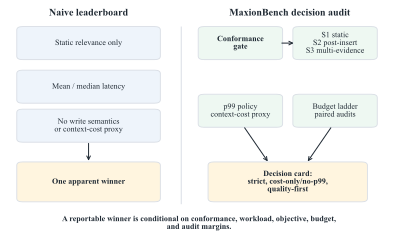
\includegraphics[width=\linewidth]{../figures/maxionbench_decision_audit_conceptual.svg}
  \caption{From leaderboard evaluation to decision audit. \sys makes a deployment choice reportable only after conformance, workload evidence, p99 policy, context-cost accounting, budget stability, and paired margins are all visible.}
  \label{fig:protocol-schematic}
\end{figure}

\subsection{Workloads}

\sys uses three workloads designed to isolate retrieval-infrastructure behavior that matters to agentic applications. S1 (single-hop static retrieval) evaluates SciFact and FiQA through local BEIR-format bundles \citep{thakur2021beir,wadden2020scifact,maia2018fiqa}; its primary quality metric is \ndcg. S2 (streaming retrieval with post-insert probes) combines a deterministic 50K-passage static background from the same source family with a CRAG-500 event stream \citep{facebookcrag}; it reports static \ndcg{} and post-insert top-10 retrievability probes at one and five seconds after insert acknowledgment. S3 (multi-evidence HotpotQA retrieval) uses \hotpotmaxionbench{}, a frozen preprocessing of the HotpotQA dev distractor split, and measures whether the retrieved top-10 contains the supporting evidence set with \ecov. \hotpotmaxionbench{} contains 7{,}405 questions; the paper-facing S3 multi-evidence matched audit uses the configured 5{,}000-query subset recorded by the run configuration.

\begin{table}[t]
\centering
\scriptsize
\setlength{\tabcolsep}{2pt}
\caption{MaxionBench workload summary. S1 single-hop and S2 streaming counts come from the processed local BEIR-format bundles under the 50K-document paper cap; S3 multi-evidence counts come from the HotpotQA-MaxionBench manifest. Cov@10 denotes \ecov{}, and all-hit@10 denotes all\_evidence\_hit@10.}
\label{tab:workload-summary}
\begin{tabularx}{\linewidth}{@{}>{\raggedright\arraybackslash}p{0.08\linewidth}>{\raggedright\arraybackslash}p{0.13\linewidth}>{\raggedright\arraybackslash}p{0.12\linewidth}>{\raggedright\arraybackslash}p{0.13\linewidth}>{\raggedright\arraybackslash}p{0.09\linewidth}>{\raggedright\arraybackslash}p{0.22\linewidth}>{\raggedright\arraybackslash}p{0.15\linewidth}@{}}
\toprule
Workload & Assets & Corpus & Queries / events & Labels & Decision role & Metrics \\
\midrule
S1 & BEIR-format SciFact + FiQA & 50{,}000 docs & 894 queries & 1{,}685 qrels & static relevance and tail-latency baseline & \ndcg{} \\
S2 & 50K BEIR background + CRAG-500 stream & 50{,}000 background + 500 inserted stream passages & 894 static queries; 500 stream events & 1{,}685 static qrels; 500 event qrels & post-insert retrievability diagnostic under a write stream & \ndcg{}; post-insert@1s/5s \\
S3 & \hotpotmaxionbench{} from HotpotQA dev distractor & 66{,}635 docs & 7{,}405 questions; 5{,}000-query matched-audit subset & 14{,}810 qrels & multi-evidence and context-cost decision stress & Cov@10; all-hit@10 \\
\bottomrule
\end{tabularx}
\end{table}

The experiments use fixed read/write-client settings so latency, throughput, and post-insert probes are comparable across engines. S1 single-hop and S3 multi-evidence evaluate read-client settings $\{1,4,8\}$. S2 streaming uses eight read clients and two serialized write clients, then probes each inserted event passage at $T+1s$ and $T+5s$, where $T$ is the time at which the adapter's insert plus flush path returns. Each workload is evaluated with two local embedding tiers, \texttt{BAAI/bge-small-en-v1.5} and \texttt{BAAI/bge-base-en-v1.5} \citep{bge}. We write bge-small and bge-base after first mention.

\subsection{Metrics and decisions}

\sys reports quality, tail latency, throughput, a normalized context-cost proxy, and stability across budget levels. Latency is measured on precomputed query vectors and times \texttt{adapter.query} plus top-k materialization, including service/container overhead inside the adapter call when applicable; offline embedding is excluded from latency and included only in the context-cost proxy. We rank latency by \maxrowp: the maximum observed p99 across the configured B2 read-client or read/write-client rows and repeats for a candidate. We report this audit statistic with the recorded hardware/runtime profile. For S1 single-hop and S2 streaming, quality is \ndcg. For S3 multi-evidence, quality is
\[
\mathrm{evidence\_coverage@k}(q)=\frac{|E(q)\cap R_k(q)|}{|E(q)|},
\]
where $E(q)$ is the gold evidence set and $R_k(q)$ is the retrieved top-$k$ set. For S2 streaming, \(\mathrm{post\_insert\_hit@10,\Delta}\) is one when the newly inserted supporting passage appears in $R_{10}(q,T+\Delta)$ for $\Delta\in\{1s,5s\}$ after the adapter's insert-plus-flush path returns. This agent-facing metric evaluates retrievability after acknowledgement; low-level index visibility is outside the metric. For S2 streaming, the strict-latency rule gates on static nDCG@10 and reports \texttt{post\_insert\_hit@10,1s} and \texttt{post\_insert\_hit@10,5s} as agent-facing write/retrieve diagnostics. We therefore interpret S2 streaming deployment choices as static-quality/cost/p99 decisions accompanied by post-insert retrievability evidence.

Within each workload and configured subset, all reportable engines evaluate the same quality query or event IDs; latency and throughput observation counts may differ because they are measured in timed windows. Paired audits join explicitly by query ID or event index. Quality differences across engines therefore reflect configured search behavior, tie handling, filtering/update semantics, and top-k materialization under the adapter contract rather than differences in the embedding model itself. In the reported MaxionBench matrix, the FAISS CPU rows have empty \texttt{index\_params} and therefore use the adapter's exact flat index; recorded \texttt{hnsw\_ef} sweep values are not consumed by that flat-index path.

The deployment rule is deliberately simple. A strict-latency survivor must pass the conformance gate, satisfy the workload quality floor recorded in the run configuration, and remain below the stated \maxrowp cap. For each workload, engine, and embedding tier, these survivors are ranked by the normalized context-cost proxy
\[
\mathrm{task\_cost\_est}=C_{\mathrm{retrieval}}+C_{\mathrm{embedding}}+c_{\mathrm{llm\_in}}\cdot N_{\mathrm{retrieved\_input\_tokens}},
\]
with lower \maxrowp and higher throughput used as tie-breaks. The report field is named \texttt{task\_cost\_est}, but the paper interprets it only as a normalized context-token cost proxy: it is not a cloud-dollar estimate. In the reported local run, \(C_{\mathrm{embedding}}=0\) for offline embeddings and \(c_{\mathrm{llm\_in}}=0.15\) is a project-defined token coefficient. The strict-latency objective selects the lowest-cost survivor under the 200 ms \maxrowp cap used as the main audit policy. The report also exposes cost-only/no-p99 and quality-first objectives because those plausible operator choices can select different configurations.

\begin{center}
\fbox{\begin{minipage}{0.92\linewidth}
\footnotesize
\textbf{Decision-card protocol.} Given engines \(E\), embedding tiers \(M\), workloads \(W\), budget levels \(B\), a p99 cap \(\tau\), and objectives \(O\), \sys runs the following audit:
\begin{enumerate}[leftmargin=*,nosep]
  \item run adapter conformance checks for each engine and exclude non-conforming rows;
  \item evaluate quality, \maxrowp, throughput, and context-cost proxy for each workload and embedding tier;
  \item rank surviving configurations under each stated objective and record strict-latency, cost-only/no-p99, and quality-first choices;
  \item compute B0/B1/B2 stability statistics and run paired audits for high-risk aggregate margins;
  \item emit a decision card with choices, margins, stability, conformance status, and interpretation notes.
\end{enumerate}
\end{minipage}}
\end{center}

\subsection{Budget ladder}

The benchmark uses three budget levels to test whether decisions are stable under shorter budgeted runs. B0 uses 10 seconds of warmup, 10 seconds of measurement, and one repeat. B1 uses 15 seconds of warmup, 30 seconds of measurement, and one repeat. B2 uses 30 seconds of warmup, 60 seconds of measurement, and two repeats. Stability is reported as Spearman rank correlation, top-1 agreement, and top-2 agreement between budget-level rankings. This design turns budget instability into a reported experimental outcome.

\section{Related work}

Information-retrieval benchmarks provide the relevance backbone for this work. MS MARCO \citep{bajaj2016msmarco}, Natural Questions \citep{kwiatkowski2019natural}, KILT \citep{petroni2021kilt}, BEIR \citep{thakur2021beir}, SciFact \citep{wadden2020scifact}, FiQA \citep{maia2018fiqa}, and HotpotQA \citep{yang2018hotpotqa} supply reusable corpora, tasks, and judgments, but they do not specify retrieval-engine conformance, write/retrieve probes, context-cost estimates, or deployment decision rules. \sys reuses labeled retrieval evidence while adding the systems and decision-audit layer needed for local infrastructure choices.

Prior work on neural retrieval and RAG motivates the agent-facing evidence layer. Sentence-BERT \citep{reimers2019sentence}, DPR \citep{karpukhin2020dense}, ColBERT \citep{khattab2020colbert}, ANCE \citep{xiong2021approximate}, E5 \citep{wang2022text}, and MTEB \citep{muennighoff2023mteb} study representation quality and retrieval-model evaluation; REALM \citep{guu2020retrieval}, RAG \citep{lewis2020retrieval}, FiD \citep{izacard2021leveraging}, RETRO \citep{borgeaud2022improving}, RAGAS \citep{es2024ragas}, and RAGBench \citep{friel2024ragbench} study retrieval-conditioned generation or RAG evaluation. These papers clarify why retrieved evidence matters, while \sys asks a lower-level deployment question: can the retrieval infrastructure surface evidence under local p99, write, and context-budget constraints?

Vector-search systems and benchmarks usually emphasize algorithmic recall, throughput, indexing configuration, and operating mode. Product quantization \citep{jegou2011product}, FLANN \citep{muja2014scalable}, HNSW \citep{malkov2020efficient}, FAISS \citep{johnson2019faiss}, ANN-Benchmarks \citep{aumuller2020ann}, the NeurIPS billion-scale ANN challenge \citep{simhadri2021bigann}, and vector-database suites such as VectorDBBench \citep{vectordbbench} expose important search-performance surfaces. These benchmarks are complementary to \sys: they characterize ANN or product performance, whereas \sys fixes an agent-facing adapter contract and ties configured search behavior to retrieval quality, post-insert top-10 retrievability, context-token cost, and deployment objectives.

Benchmark methodology and agent-memory work motivate the reporting style. MLPerf Inference \citep{reddi2019mlperf} emphasizes rules and reproducible system comparisons; HELM \citep{liang2023helm} emphasizes multi-metric transparency; datasheets \citep{gebru2021datasheets} and Croissant metadata \citep{mlcommons2024croissant} motivate explicit dataset documentation; and tail-latency work motivates high-percentile latency reporting \citep{dean2013tail}. AgentBench \citep{liu2023agentbench}, MemGPT \citep{packer2023memgpt}, LongMemEval \citep{wu2024longmemeval}, and LoCoMo \citep{maharana2024locomo} evaluate agent behavior or long-term memory. \sys applies the reporting discipline to retrieval stores used as local agent memory.

\FloatBarrier
\section{Experiments}
\suppressfloats[t]

\subsection{Evaluation validation}

The reported results come from a frozen evaluation snapshot included with the supplementary material. The snapshot contains raw run records, generated figures, the \hotpotmaxionbench{} manifest and checksums, and the conformance matrix. A strict-schema validation pass checked 72 run records and returned zero errors. Appendix Table~\ref{tab:portable-support} reports passing conformance and behavior-card coverage for FAISS CPU, LanceDB in-process, pgvector, and Qdrant; LanceDB service is excluded because it has no conformance row.

The supplementary material is intended to make each paper claim traceable. It contains the benchmark code, validation summary, conformance matrix, generated tables and figures, query-level paired-audit summaries, checksums, \hotpotmaxionbench{} Croissant-style metadata \citep{mlcommons2024croissant}, and a claim-evidence map. The main results below are tied to the recorded configs, conformance gate, objectives, and budget levels.

\subsection{Decision audit results}

We organize results around four deployment-audit questions. First, under the default 200 ms \maxrowp policy, FAISS CPU with bge-small is the policy-selected strict-latency configuration for all three workloads. Second, this decision is objective-sensitive: removing the p99 cap or optimizing quality changes selected configurations. Third, paired audits separate clear margins from aggregate near-ties. Fourth, budget stability is workload-dependent, so short screening runs cannot always replace B2 decisions.

\begin{figure}[t]
  \centering
  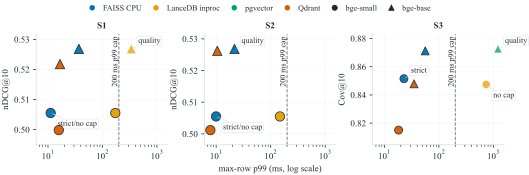
\includegraphics[width=\linewidth]{../figures/portable_decision_surface.pdf}
  \caption{Decision surface for the B2 audit. The strict 200 ms \maxrowp policy selects FAISS CPU/bge-small for S1 single-hop, S2 streaming, and S3 multi-evidence, but the no-p99 and quality-first markers show that the selection is conditional on objective and policy. Each panel uses a workload-specific zoomed y-axis.}
  \label{fig:decision-surface}
\end{figure}

\input{tables/neurips_main_results}

Table~\ref{tab:portable-main-results} is a strict-latency deployment-card summary. Under the 200 ms \maxrowp threshold, all three workloads select FAISS CPU with \texttt{BAAI/bge-small-en-v1.5}. The FAISS rows are exact FlatIP local-baseline rows, while the other rows include the configured store and adapter overheads; the table reports the decision under the recorded local runtime profile. The S1 single-hop selected row reaches \ndcg{} 0.506 with a 95\% confidence interval of 0.494--0.516 and \maxrowp 11.2 ms. S2 streaming selects the same engine and embedding, with \ndcg{} 0.506, \postinsertfive{} 0.830, and \maxrowp 10.0 ms. S3 multi-evidence selects FAISS CPU with \texttt{BAAI/bge-small-en-v1.5} at \ecov{} 0.852 and \maxrowp 22.8 ms.

S2 streaming measures agent-facing post-insert top-10 retrievability. S1 single-hop and the static-retrieval component of S2 streaming use the same 894-query BEIR-format evaluation pool under the 50K-document cap, which is why their static \ndcg{} and packed-token summaries can match. S2 streaming adds CRAG-500 write/retrieve probes after the adapter insert-plus-flush path returns. Across two B2 strict-choice repeats with 500 events each, 830 of 1{,}000 post-insert observations are retrieved by the 1s probe; no additional observations recover by 5s, leaving 170 of 1{,}000 absent at the 5s probe. Appendix Figure~\ref{fig:s2-postinsert}, Appendix Table~\ref{tab:s2-write-diagnostics}, and Appendix Table~\ref{tab:s2-post-insert-examples} report the fixed-probe diagnostics and example event/query/document IDs.

The benchmark-design ablation is reported in Appendix Table~\ref{tab:decision-error-ablation}. Its main implication is that removing any audit component changes the interpretation: the p99 gate separates strict-latency decisions from cost-only/no-p99 choices, objective separation prevents quality-first rows from being conflated with strict-latency rows, budget reporting exposes unstable S1 single-hop and S2 streaming screening runs, paired audits prevent aggregate near-ties from being overclaimed, and conformance filtering keeps unsupported service rows out of paper-facing tables.

\input{tables/portable_decision_table}

Table~\ref{tab:portable-decision-table} and Figure~\ref{fig:decision-surface} show objective sensitivity directly. The strict-latency and cost-only/no-p99 objectives agree for S1 single-hop and S2 streaming, but S3 multi-evidence shifts to LanceDB in-process with \texttt{BAAI/bge-small-en-v1.5} when the p99 cap is removed. Quality-first decisions differ more strongly: LanceDB in-process with \texttt{BAAI/bge-base-en-v1.5} leads S1 single-hop, FAISS CPU with \texttt{BAAI/bge-base-en-v1.5} leads S2 streaming, and the aggregate quality-first rule selects pgvector with \texttt{BAAI/bge-base-en-v1.5} for S3 multi-evidence. The threshold sweep makes the 200 ms policy explicit and auditable.

\begin{figure}[t]
  \centering
  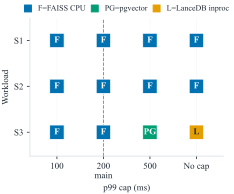
\includegraphics[width=0.62\linewidth]{../figures/portable_mvd_sensitivity.pdf}
  \caption{S3 multi-evidence is sensitive to relaxing the p99 policy, while S1 single-hop and S2 streaming keep the same policy-selected engine across the reported thresholds. This threshold sweep shows how MaxionBench reports decisions under stated local policies.}
  \label{fig:p99-sensitivity}
\end{figure}

\begin{figure}[t]
  \centering
  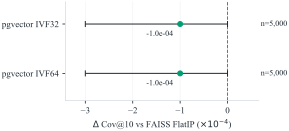
\includegraphics[width=0.72\linewidth]{../figures/s3_paired_audit_forest.pdf}
  \caption{Matched S3 multi-evidence paired audit. Against FAISS exact FlatIP on the same 5{,}000 bge-base queries, pgvector IVF32 and IVF64 have paired \ecov{} deltas whose 95\% intervals include zero, so the aggregate pgvector quality-first row shows no detectable advantage under matched queries.}
  \label{fig:s3-paired-audit}
\end{figure}

The S3 multi-evidence quality-first margin is the highest-risk aggregate claim, so we audit it with matched queries. Using all B2 rows, pgvector-base exceeds FAISS-base by only 0.00016 \ecov{} with an aggregate-row bootstrap interval of -0.00280 to 0.00304. The matched audit in Figure~\ref{fig:s3-paired-audit} removes even that apparent edge: pgvector IVF32 and IVF64 are each 0.0001 \ecov{} below FAISS exact FlatIP on the 5{,}000-query matched-audit subset, with paired intervals including zero. We therefore report no detectable pgvector advantage at this sample size rather than a quality win. Appendix Table~\ref{tab:s3-paired-quality} gives the numeric rows, and Appendix Table~\ref{tab:s3-all-evidence-hit} records the stricter binary all\_evidence\_hit@10 audit.

Appendix Table~\ref{tab:strict-decision-margins} makes the strict-latency decision margins explicit. For S1 single-hop and S2 streaming, FAISS CPU with \texttt{BAAI/bge-small-en-v1.5} matches the closest LanceDB in-process candidate on relevance quality and cost, so the deployment rule resolves the tie by lower \maxrowp and higher throughput. For S3 multi-evidence, Qdrant with \texttt{BAAI/bge-small-en-v1.5} is the nearest strict-cost alternative but is more expensive and lower quality, even though its \maxrowp is 4.6 ms lower in the repeat-aware table. The highest-quality strict-latency S3 multi-evidence option remains FAISS CPU with \texttt{BAAI/bge-base-en-v1.5}, which improves \ecov{} by 0.020 over \texttt{BAAI/bge-small-en-v1.5} but increases the normalized context-cost proxy by 0.704 and \maxrowp by 33.4 ms on the B2 audit rows.

The normalized context-cost proxy is stable under the coefficient sensitivity tested in the supplementary analysis. Appendix Table~\ref{tab:cost-sensitivity} rescales only \(c_{\mathrm{llm\_in}}\) from 0.1$\times$ to 10$\times$ and leaves all strict choices unchanged: S1 single-hop and S2 streaming have identical retrieved-token counts for the strict choice and nearest strict-cost competitor, while S3 multi-evidence FAISS/bge-small retrieves slightly fewer tokens than Qdrant/bge-small. Appendix Table~\ref{tab:latency-distribution} reports p50, p95, mean p99, and the min--max p99 range over B2 run rows for the recorded hardware/runtime profile.

\begin{figure}[t]
  \centering
  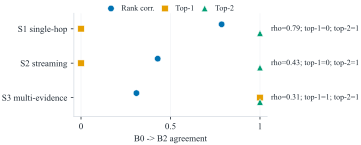
\includegraphics[width=0.62\linewidth]{../figures/portable_budget_stability.pdf}
  \caption{Budget stability is workload-dependent. B0 screening fails to preserve B2 top-1 choices for S1 single-hop and S2 streaming, while S3 multi-evidence preserves top-1 despite low full-rank Spearman correlation.}
  \label{fig:budget-effects}
\end{figure}

The budget analysis measures how much evidence is enough. B0-to-B2 top-1 agreement is zero for S1 single-hop and S2 streaming, with Spearman correlations 0.79 and 0.43, respectively. S3 multi-evidence has top-1 agreement of one but Spearman correlation 0.31, meaning that the selected strict-latency row is stable while lower-ranked alternatives remain noisy. The resulting decision card includes the budget level and stability statistics used to reach each recommendation.

\subsection{Targeted replication checks}

Targeted same-machine reruns support the decision-level conclusions and quantify tail-latency variation. Appendix Table~\ref{tab:strict-faiss-repeat-audit} shows that the strict FAISS CPU/bge-small choices reproduce the relevant quality values and remain under the 200 ms policy; the S3 multi-evidence bge-base rerun and Figure~\ref{fig:s3-paired-audit} support the objective-sensitivity story; and Appendix Table~\ref{tab:s2-competitor-check} reports a larger FAISS-versus-Qdrant S2 streaming paired check that finds no Qdrant quality or post-insert retrievability advantage. A final S3 local-scale check on the 66{,}635-document \hotpotmaxionbench{} corpus compares exact FAISS CPU and LanceDB in-process over the same 5{,}000-query cap: FAISS reports \ecov{} 0.8515 and p99 17.4 ms, while LanceDB reports \ecov{} 0.8514 and p99 172.4 ms; the existing validated Qdrant row reports \ecov{} 0.8117 and p99 21.0 ms. To isolate corpus-size effects, Appendix Table~\ref{tab:faiss-scale-stress} adds a controlled FAISS vector-scale stress check: at 1M vectors, exact FlatIP remains under 200 ms p99, but IVF reaches p99 9.45 ms with recall@10 0.9994 against FlatIP. Appendix Table~\ref{tab:cross-engine-scale-stress} adds a non-FAISS sanity check on the same vector construction: Qdrant HNSW reaches recall@10 0.9994 at 250K vectors with p99 8.91 ms and remains fully indexed at 1M vectors with recall@10 0.9994 and p99 10.05 ms. Read against the FAISS scale rows, the fully indexed Qdrant row shows that the local ordering can change by 250K vectors: FAISS exact is faster at 66K, while Qdrant HNSW is faster at 250K at near-exact recall. These checks support the local 50K--66K exact-baseline finding while showing why the paper does not present that ranking as production-scale evidence.

\FloatBarrier
\section{Experimental boundaries and broader impact}

\sys reports CPU-only, single-node retrieval-memory decisions for FAISS CPU, LanceDB in-process, pgvector, and Qdrant under recorded adapter settings. The current engine ranking is local evidence at 50K--66K corpus scale, where FAISS exact FlatIP is a strong baseline; it should not be interpreted as a production-scale ranking. The vector-scale stress checks extend the corpus-size envelope to 1M vectors with deterministic random unit-vector distractors and a fully indexed Qdrant HNSW sanity row, but they remain vector-only checks rather than full task-quality, post-insert, persistence, or distributed-operation evaluations. Engine-level quality differences are configured-search differences under the MaxionBench adapter settings, and future sweeps can vary larger corpora, GPU modes, higher probe and ef settings, cloud or second-machine profiles, and distributed stores within the same adapter contract. The broader impact is methodological: a reproducible benchmark can help operators choose retrieval infrastructure while keeping quality, post-insert retrievability, objective choice, budget level, and paired margins visible.

\section{Conclusion}

\sys frames retrieval infrastructure for agentic AI as an auditable deployment decision rather than a leaderboard. The key idea is to report a configuration only after it passes a fixed adapter contract, then expose workload quality, post-insert top-10 retrievability, \maxrowp latency, normalized context-cost proxy, budget stability, objective sensitivity, and paired margins in one decision card. The experimental evidence shows why that audit matters: the strict 200 ms policy selects FAISS CPU/bge-small for S1 single-hop, S2 streaming, and S3 multi-evidence, but alternative objectives change decisions, S1 single-hop and S2 streaming are tail-latency tie-breaks, the S3 multi-evidence pgvector aggregate edge is indistinguishable under matched queries, and short B0 runs do not preserve all B2 decisions. The operational conclusion is that retrieval-memory deployment choices are more credible when their conformance, objective, budget, and decision margins are explicit.


\FloatBarrier
\clearpage
\bibliographystyle{plainnat}
\bibliography{references}

\clearpage
\appendix
\section{Reproducibility details}
\suppressfloats[t]

The supplementary material provides the workflow instructions used to reproduce the benchmark setup, data preparation, B0--B2 runs, final report generation, and strict-schema validation. The frozen evaluation snapshot used by this manuscript contains raw run records, generated paper figures, \hotpotmaxionbench{} metadata, and conformance evidence. The validation summary reports \texttt{"pass": true}, \texttt{"error\_count": 0}, and \texttt{"run\_dirs\_checked": 72}.

The validated MaxionBench matrix contains 72 run-result tables, including 24 B2 result tables with matching run metadata. The public submission records a CPU-only local runtime profile and omits machine-specific identifiers. The reported matrix uses CPU rows throughout. \hotpotmaxionbench{} contains 66{,}635 documents, 7{,}405 questions, and 14{,}810 qrels; the verified manifest fields are \texttt{doc\_count=66635}, \texttt{question\_count=7405}, and \texttt{qrel\_count=14810}. The S3 multi-evidence matched audit uses the configured 5{,}000-query subset cap recorded in the run configuration, while the full \hotpotmaxionbench{} manifest remains part of the supplement. The HotpotQA-MaxionBench checksum manifest stores SHA-256 checksums for the corpus, queries, qrels, metadata, and manifest.

The supplementary package also includes an artifact card, a consistency verifier, and Croissant-style metadata for \hotpotmaxionbench{}. The verifier checks that the manuscript, evaluation manifest, paper-facing tables, paired-audit summaries, and metadata files are present and internally consistent; the Croissant metadata records the corpus, query, and qrel files, their intended evaluation use, and the license/provenance boundary inherited from HotpotQA.

\section{Audit tables}
\suppressfloats[t]

\input{tables/cost_formula}
\input{tables/cost_sensitivity}
\input{tables/latency_distribution}
\input{tables/strict_faiss_repeat_audit}
% Auto-generated by maxionbench.reports.portable_exports.
\begin{table}[t]
\centering
\small
\setlength{\tabcolsep}{3.5pt}
\caption{Protocol components whose omission changes or weakens deployment conclusions.}
\label{tab:decision-error-ablation}
\resizebox{\linewidth}{!}{%
\begin{tabular}{lll}
\toprule
Missing component & Wrong conclusion caused by omission & Evidence \\
\midrule
p99 latency gate & S3 multi-evidence cost-only/no-p99 choice shifts to lancedb-inproc/bge-small instead of faiss-cpu/bge-small & decision table and threshold-sensitivity panel \\
Objective separation & Quality-first decisions differ from strict-latency decisions on S1 single-hop, S2 streaming, and S3 multi-evidence & decision table \\
Budget ladder & B0 screening fails to preserve B2 top-1 decisions for S1 single-hop and S2 streaming & budget-stability figure and decision table \\
Paired S3 multi-evidence audit & pgvector/bge-base appears quality-first for S3 multi-evidence, but the matched 5,000-query audit removes the substantive margin & S3 multi-evidence paired audit table \\
Paired S2 streaming competitor audit & Paired check finds no Qdrant quality or post-insert retrievability advantage & S2 streaming competitor audit table \\
Conformance gate & Engines enter paper-facing result tables only after passing local conformance rows & benchmark setup, support table, and evaluation validation \\
\bottomrule
\end{tabular}
}
\end{table}

\input{tables/decision_surface}
\input{tables/strict_decision_margins}
\begin{figure}[t]
  \centering
  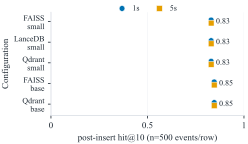
\includegraphics[width=0.70\linewidth]{../figures/portable_s2_post_insert_retrievability.svg}
  \caption{S2 streaming post-insert top-10 retrievability for B2 strict survivors. One- and five-second probes overlap in the validated rows, showing no additional recoveries between the fixed probes.}
  \label{fig:s2-postinsert}
\end{figure}
\input{tables/s2_write_diagnostics}
\input{tables/s2_post_insert_examples}
\input{tables/portable_support_table}
\input{tables/engine_configuration}
\input{tables/s3_paired_quality}
\input{tables/s3_all_evidence_hit}
\input{tables/s1_s2_lancedb_paired}
\input{tables/s2_competitor_check}
% Auto-generated by maxionbench.reports.portable_exports.
\begin{table}[t]
\centering
\small
\setlength{\tabcolsep}{3.5pt}
\caption{Quality floors and strict-p99 B2 survivors used by the strict-latency decision rule. Floor values come from the benchmark run configuration and match the report generator's floor rule. S2 streaming post-insert metrics are diagnostics in the decision rule, not additional hard gates.}
\label{tab:quality-floor-survivors}
\resizebox{\linewidth}{!}{%
\begin{tabular}{lllrr}
\toprule
Workload & Quality metric & Quality floor source & Floor value & Strict-p99 survivors \\
\midrule
S1 single-hop & nDCG@10 & configured quality floor & 0.25 & 5 \\
S2 streaming & nDCG@10 plus post-insert reporting & configured quality floor & 0.25 & 5 \\
S3 multi-evidence & evidence\_coverage@10 & configured quality floor & 0.30 & 4 \\
\bottomrule
\end{tabular}
}
\end{table}


\FloatBarrier

\section{Claim-evidence map}

\begin{table}[t]
\centering
\small
\setlength{\tabcolsep}{3.5pt}
\caption{Reviewer-facing evidence map. The main claims are framed as benchmark and decision-audit claims with stated objective and policy conditions.}
\label{tab:evidence-strength}
\resizebox{\linewidth}{!}{%
\begin{tabular}{llll}
\toprule
Claim & Main evidence & Residual risk & Paper stance \\
\midrule
Conformance-gated reporting & 72 strict-schema run dirs; support table & Adapter coverage follows the recorded local matrix & Supported protocol claim \\
Strict-latency decisions & Figure~\ref{fig:decision-surface}; main and decision tables; margin table & Recorded CPU-only runtime profile & Deployment decision evidence \\
Strict FAISS repeat evidence & Same-machine repeat audit in Table~\ref{tab:strict-faiss-repeat-audit} & Repeats report tail-latency variation under the recorded runtime profile & Supplementary robustness check \\
Decision surface is visible & B2 strict survivors and objective rows in Figure~\ref{fig:decision-surface} and Table~\ref{tab:decision-surface} & Full matrix remains appendix and supplementary material & Anti-cherry-picking evidence \\
S2 streaming competitor check & S2 streaming diagnostics in Tables~\ref{tab:s2-write-diagnostics}--\ref{tab:s2-post-insert-examples}; larger same-machine paired S2 streaming check in Table~\ref{tab:s2-competitor-check} & Fixed 1s/5s probes and ID-level observations & Competitor quality/post-insert audit \\
S3 multi-evidence pgvector quality edge is indistinguishable under matched queries & 5{,}000-query paired audit against FAISS exact FlatIP in Figure~\ref{fig:s3-paired-audit} and Table~\ref{tab:s3-paired-quality} & Higher ef/probe service sweeps are extension rows & Objective-sensitivity audit \\
Budget stability is workload-dependent & Figure~\ref{fig:budget-effects}; B0-to-B2 top-1 and Spearman stats & Lower ranks remain noisy & Report budgets explicitly \\
\bottomrule
\end{tabular}
}
\end{table}


\begin{itemize}[leftmargin=*]
  \item Claim: \sys is conformance-gated. Evidence: Table~\ref{tab:portable-support} reports passing conformance and behavior cards for all included engines, and the report excludes LanceDB service because conformance is missing.
  \item Claim: the paper contributes a reusable decision-audit protocol rather than only a benchmark implementation. Evidence: the decision-card protocol in Section~2.3 defines the conformance gate, workload evaluation, objective-specific ranking, budget-stability check, paired audit, and emitted card fields.
  \item Claim: strict 200 ms \maxrowp{} deployment selects FAISS CPU with \texttt{BAAI/bge-small-en-v1.5} for S1 single-hop, S2 streaming, and S3 multi-evidence. Evidence: Table~\ref{tab:portable-main-results} and Table~\ref{tab:portable-decision-table}.
  \item Claim: supplementary same-machine repeat evidence supports the strict FAISS CPU/bge-small decisions. Evidence: Table~\ref{tab:strict-faiss-repeat-audit} summarizes completed local repeat rows for S1 single-hop, S2 streaming, and S3 multi-evidence.
  \item Claim: the selected rows are shown against the full decision surface. Evidence: Figure~\ref{fig:decision-surface} and Table~\ref{tab:decision-surface} show all B2 strict survivors plus objective winners outside the strict survivor set.
  \item Claim: strict decisions have different margins across workloads. Evidence: Table~\ref{tab:strict-decision-margins} shows S1 single-hop and S2 streaming as cost/quality ties resolved by latency and S3 multi-evidence as lower-cost and higher-quality than the next strict-cost candidate.
  \item Claim: objective choice changes deployment conclusions. Evidence: Table~\ref{tab:portable-decision-table} shows different quality-first winners for all workloads and a cost-only/no-p99 shift for S3 multi-evidence.
  \item Claim: the S3 multi-evidence quality-first pgvector result is indistinguishable from FAISS under matched queries. Evidence: Figure~\ref{fig:s3-paired-audit} and Table~\ref{tab:s3-paired-quality} report a matched-query audit over the 5{,}000-query S3 multi-evidence matched-audit subset in which pgvector trails the FAISS exact FlatIP baseline by 0.0001 \ecov{} with paired 95\% interval [-0.0003, 0.0000].
  \item Claim: the S2 streaming competitor audit finds no Qdrant quality or post-insert retrievability advantage. Evidence: Table~\ref{tab:s2-write-diagnostics} summarizes B2 post-insert diagnostics, Table~\ref{tab:s2-post-insert-examples} gives strict-choice success/miss examples and counts, and Table~\ref{tab:s2-competitor-check} reports a larger same-machine paired check with 1{,}788 matched quality observations and 200 matched post-insert events.
  \item Claim: budget stability is workload-dependent. Evidence: Figure~\ref{fig:budget-effects}; B0-to-B2 top-1 agreement is 0 for S1 single-hop and S2 streaming and 1 for S3 multi-evidence, with Spearman correlations 0.79, 0.43, and 0.31.
\end{itemize}

\FloatBarrier


\input{checklist}

\end{document}
